\documentclass{standalone}
\usepackage{tikz}
\usetikzlibrary{patterns, positioning}
\usepackage[sfdefault]{ClearSans} %% option 'sfdefault' activates Clear Sans as the default text font
\usepackage[T1]{fontenc}

\begin{document}
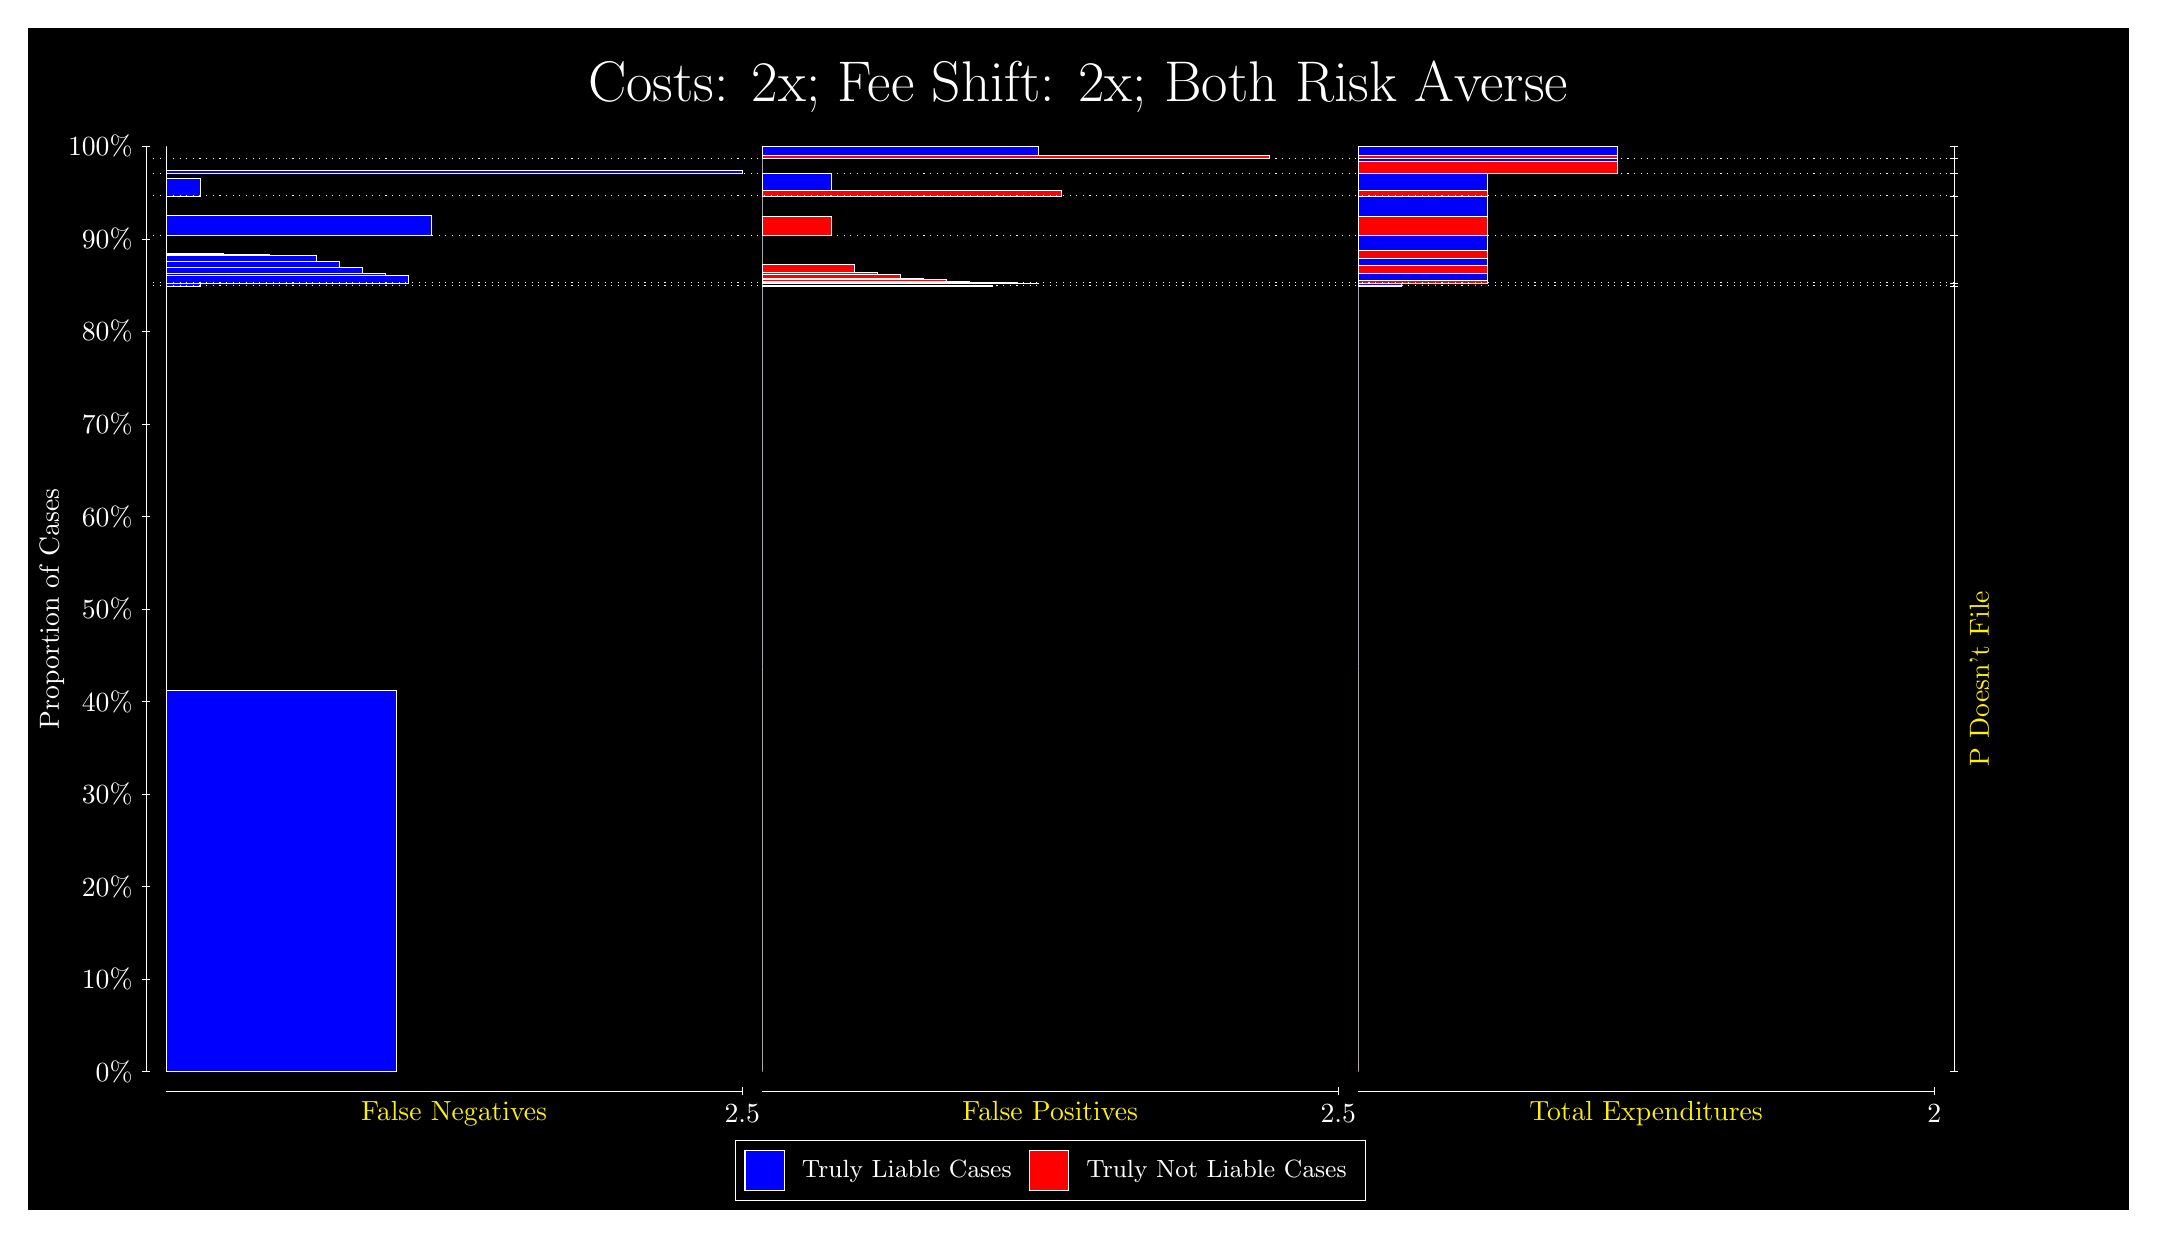
\begin{tikzpicture}
\draw[fill=black] (0,0) rectangle (26.667,15);
\draw[text=white] (0,13.5) rectangle (26.667,15) node[midway] {\huge Costs: 2x; Fee Shift: 2x; Both Risk Averse};
\draw[white, very thin] (1.5,1.75) -- (1.5,13.5);
\node[rotate=90, text=white, anchor=center] at (0.3, 7.625) {Proportion of Cases};
\draw[white, very thin] (1.45,1.75) -- (1.55,1.75);
\node[text=white, anchor=east] at (1.45, 1.75) {0\%};
\draw[white, very thin] (1.45,2.925) -- (1.55,2.925);
\node[text=white, anchor=east] at (1.45, 2.925) {10\%};
\draw[white, very thin] (1.45,4.1) -- (1.55,4.1);
\node[text=white, anchor=east] at (1.45, 4.1) {20\%};
\draw[white, very thin] (1.45,5.275) -- (1.55,5.275);
\node[text=white, anchor=east] at (1.45, 5.275) {30\%};
\draw[white, very thin] (1.45,6.45) -- (1.55,6.45);
\node[text=white, anchor=east] at (1.45, 6.45) {40\%};
\draw[white, very thin] (1.45,7.625) -- (1.55,7.625);
\node[text=white, anchor=east] at (1.45, 7.625) {50\%};
\draw[white, very thin] (1.45,8.8) -- (1.55,8.8);
\node[text=white, anchor=east] at (1.45, 8.8) {60\%};
\draw[white, very thin] (1.45,9.975) -- (1.55,9.975);
\node[text=white, anchor=east] at (1.45, 9.975) {70\%};
\draw[white, very thin] (1.45,11.15) -- (1.55,11.15);
\node[text=white, anchor=east] at (1.45, 11.15) {80\%};
\draw[white, very thin] (1.45,12.325) -- (1.55,12.325);
\node[text=white, anchor=east] at (1.45, 12.325) {90\%};
\draw[white, very thin] (1.45,13.5) -- (1.55,13.5);
\node[text=white, anchor=east] at (1.45, 13.5) {100\%};

\draw[white, very thin] (24.457,1.75) -- (24.457,13.5);
\draw[white, very thin] (24.407,1.75) -- (24.507,1.75);
\node[anchor=west] at (24.407, 1.75) {};
\draw[white, very thin] (24.407,11.728) -- (24.507,11.728);
\node[anchor=west] at (24.407, 11.728) {};
\draw[white, very thin] (24.407,11.765) -- (24.507,11.765);
\node[anchor=west] at (24.407, 11.765) {};
\draw[white, very thin] (24.407,12.372) -- (24.507,12.372);
\node[anchor=west] at (24.407, 12.372) {};
\draw[white, very thin] (24.407,12.871) -- (24.507,12.871);
\node[anchor=west] at (24.407, 12.871) {};
\draw[white, very thin] (24.407,13.159) -- (24.507,13.159);
\node[anchor=west] at (24.407, 13.159) {};
\draw[white, very thin] (24.407,13.344) -- (24.507,13.344);
\node[anchor=west] at (24.407, 13.344) {};
\draw[white, very thin] (24.407,13.5) -- (24.507,13.5);
\node[anchor=west] at (24.407, 13.5) {};

\draw[white, very thin, fill=blue] (1.75,1.75) rectangle (4.6775,6.5866);
\draw[white, very thin, fill=red] (1.75,6.5866) rectangle (1.75,11.728);
\draw[white, very thin, fill=blue] (1.75,11.728) rectangle (2.1891,11.761);
\draw[white, very thin, fill=red] (1.75,11.761) rectangle (1.75,11.765);
\draw[white, very thin, fill=blue] (1.75,11.765) rectangle (4.8239,11.859);
\draw[white, very thin, fill=blue] (1.75,11.859) rectangle (4.5312,11.883);
\draw[white, very thin, fill=blue] (1.75,11.883) rectangle (4.2384,11.967);
\draw[white, very thin, fill=blue] (1.75,11.967) rectangle (3.9457,12.038);
\draw[white, very thin, fill=blue] (1.75,12.038) rectangle (3.6529,12.11);
\draw[white, very thin, fill=blue] (1.75,12.11) rectangle (3.3602,12.12);
\draw[white, very thin, fill=blue] (1.75,12.12) rectangle (3.0674,12.129);
\draw[white, very thin, fill=blue] (1.75,12.129) rectangle (2.7746,12.134);
\draw[white, very thin, fill=blue] (1.75,12.134) rectangle (2.4819,12.139);
\draw[white, very thin, fill=red] (1.75,12.139) rectangle (1.75,12.372);
\draw[white, very thin, fill=blue] (1.75,12.372) rectangle (5.1167,12.63);
\draw[white, very thin, fill=red] (1.75,12.63) rectangle (1.75,12.871);
\draw[white, very thin, fill=blue] (1.75,12.871) rectangle (2.1891,13.088);
\draw[white, very thin, fill=red] (1.75,13.088) rectangle (1.75,13.159);
\draw[white, very thin, fill=blue] (1.75,13.159) rectangle (9.0689,13.195);
\draw[white, very thin, fill=red] (1.75,13.195) rectangle (1.75,13.344);
\draw[white, very thin, fill=red] (1.75,13.344) rectangle (1.75,13.38);
\draw[white, very thin, fill=blue] (1.75,13.38) rectangle (1.75,13.5);
\draw[white, very thin, fill=red] (9.3189,1.75) rectangle (9.3189,6.8914);
\draw[white, very thin, fill=blue] (9.3189,6.8914) rectangle (9.3189,11.728);
\draw[white, very thin, fill=red] (9.3189,11.728) rectangle (12.246,11.732);
\draw[white, very thin, fill=blue] (9.3189,11.732) rectangle (9.3189,11.765);
\draw[white, very thin, fill=red] (9.3189,11.765) rectangle (12.832,11.767);
\draw[white, very thin, fill=red] (9.3189,11.767) rectangle (12.539,11.77);
\draw[white, very thin, fill=red] (9.3189,11.77) rectangle (12.246,11.775);
\draw[white, very thin, fill=red] (9.3189,11.775) rectangle (11.954,11.781);
\draw[white, very thin, fill=red] (9.3189,11.781) rectangle (11.661,11.806);
\draw[white, very thin, fill=red] (9.3189,11.806) rectangle (11.368,11.829);
\draw[white, very thin, fill=red] (9.3189,11.829) rectangle (11.075,11.872);
\draw[white, very thin, fill=red] (9.3189,11.872) rectangle (10.783,11.895);
\draw[white, very thin, fill=red] (9.3189,11.895) rectangle (10.49,11.998);
\draw[white, very thin, fill=blue] (9.3189,11.998) rectangle (9.9044,12.002);
\draw[white, very thin, fill=blue] (9.3189,12.002) rectangle (9.6116,12.007);
\draw[white, very thin, fill=blue] (9.3189,12.007) rectangle (9.3189,12.372);
\draw[white, very thin, fill=red] (9.3189,12.372) rectangle (10.197,12.613);
\draw[white, very thin, fill=blue] (9.3189,12.613) rectangle (9.3189,12.871);
\draw[white, very thin, fill=red] (9.3189,12.871) rectangle (13.125,12.942);
\draw[white, very thin, fill=blue] (9.3189,12.942) rectangle (10.197,13.159);
\draw[white, very thin, fill=red] (9.3189,13.159) rectangle (9.3189,13.308);
\draw[white, very thin, fill=blue] (9.3189,13.308) rectangle (9.3189,13.344);
\draw[white, very thin, fill=red] (9.3189,13.344) rectangle (15.759,13.38);
\draw[white, very thin, fill=blue] (9.3189,13.38) rectangle (12.832,13.5);
\draw[white, very thin, fill=red] (16.888,1.75) rectangle (16.888,6.8914);
\draw[white, very thin, fill=blue] (16.888,6.8914) rectangle (16.888,11.728);
\draw[white, very thin, fill=red] (16.888,11.728) rectangle (17.437,11.732);
\draw[white, very thin, fill=blue] (16.888,11.732) rectangle (17.437,11.765);
\draw[white, very thin, fill=red] (16.888,11.765) rectangle (18.534,11.797);
\draw[white, very thin, fill=blue] (16.888,11.797) rectangle (18.534,11.883);
\draw[white, very thin, fill=red] (16.888,11.883) rectangle (18.534,11.985);
\draw[white, very thin, fill=blue] (16.888,11.985) rectangle (18.534,12.079);
\draw[white, very thin, fill=red] (16.888,12.079) rectangle (18.534,12.178);
\draw[white, very thin, fill=blue] (16.888,12.178) rectangle (18.534,12.372);
\draw[white, very thin, fill=red] (16.888,12.372) rectangle (18.534,12.613);
\draw[white, very thin, fill=blue] (16.888,12.613) rectangle (18.534,12.871);
\draw[white, very thin, fill=red] (16.888,12.871) rectangle (18.534,12.942);
\draw[white, very thin, fill=blue] (16.888,12.942) rectangle (18.534,13.159);
\draw[white, very thin, fill=red] (16.888,13.159) rectangle (20.181,13.308);
\draw[white, very thin, fill=blue] (16.888,13.308) rectangle (20.181,13.344);
\draw[white, very thin, fill=red] (16.888,13.344) rectangle (20.181,13.38);
\draw[white, very thin, fill=blue] (16.888,13.38) rectangle (20.181,13.5);
\draw[white, dotted] (1.5,11.728) -- (24.457,11.728);
\draw[white, dotted] (1.5,11.765) -- (24.457,11.765);
\draw[white, dotted] (1.5,12.372) -- (24.457,12.372);
\draw[white, dotted] (1.5,12.871) -- (24.457,12.871);
\draw[white, dotted] (1.5,13.159) -- (24.457,13.159);
\draw[white, dotted] (1.5,13.344) -- (24.457,13.344);
\draw[white, very thin] (1.75,1.5) -- (9.0689,1.5);
\node[text=yellow, anchor=north] at (5.4094, 1.5) {False Negatives};
\draw[white, very thin] (9.0689,1.45) -- (9.0689,1.55);
\node[text=white, anchor=north] at (9.0689, 1.45) {2.5};

\draw[white, very thin] (9.3189,1.5) -- (16.638,1.5);
\node[text=yellow, anchor=north] at (12.978, 1.5) {False Positives};
\draw[white, very thin] (16.638,1.45) -- (16.638,1.55);
\node[text=white, anchor=north] at (16.638, 1.45) {2.5};

\draw[white, very thin] (16.888,1.5) -- (24.207,1.5);
\node[text=yellow, anchor=north] at (20.547, 1.5) {Total Expenditures};
\draw[white, very thin] (24.207,1.45) -- (24.207,1.55);
\node[text=white, anchor=north] at (24.207, 1.45) {2};

\node[text=yellow, centered, rotate=90] at (24.777, 6.739) {P Doesn't File};







\draw (12.978300999999998,1.5) node[draw=none] (baseCoordinate) {};
\begin{scope}[align=center]
        \matrix[scale=0.5, draw=white, below=0.5cm of baseCoordinate, nodes={draw}, column sep=0.1cm]{
            \node[rectangle, draw, minimum width=0.5cm, minimum height=0.5cm, fill=blue] {}; &
            \node[draw=none, font=\small, text=white] (B) {Truly Liable Cases}; &
            \node[rectangle, draw, minimum width=0.5cm, minimum height=0.5cm, fill=red] {}; &
            \node[draw=none, font=\small, text=white] (B) {Truly Not Liable Cases}; \\
            };
\end{scope}

\end{tikzpicture}
\end{document}